\chapter{Predictive Analytics im öffentlichen Sektor}

Die Methode des Forecasting hat (bisher) noch keinen bedeutenden Durchbruch in
der breiten Öffentlichkeit gehabt\footnote{
Politiker, Experten und Kommentatoren formulieren keine subjektiven Wahrscheinlichkeiten und
niemand verwendet den Brier Score (oder ein anderes Maß), um die Genauigkeit ihrer Prognosen
zu prüfen. 
}. Es gibt Stimmen, die behaupten, dass ein immenser Widerstand gegen die
Einführung dieser Methode zu erwarten ist. Teilweise deutet sich sogar eine
Unmöglichkeit dieser Aufgabe an. 
Beim Thema Forecasting ist es Tetlock selbst, der sich skeptisch äußert. Er
benennt den Widerstand der Experten als die größte Barriere zur Einführung der
neuen Methodik (\emph{the most daunting of all the barriers to implementation},
vgl. \cite{Tetlock}, S.~235). Jackson und Reichin vertreten eine ähnliche
Auffassung (vgl. \cite{Jackson}, S.~295). 

Für Predictive Analytics sind die Prognosen optimistischer (vgl. \cite{Mauerer}).
Allerdings ist zweifelhaft, ob Top Manager \emph{ihre} Entscheidungen mit Hilfe
von Predictive Analytics Methoden treffen.
Unternehmen behaupten zwar, dass strategische Entscheidungen mit Hilfe von Predictive Analytics
unterstützt werden sollen (vgl. \cite{Mauerer}, S.~2), die konkreten Anwendungsbeispiele deuten
aber darauf hin, dass hauptsächlich operative Abteilungen (wie z. B. der Kauf und Verkauf von
Gütern) betroffen sind.

Somit deutet sich die Frage an, ob grundsätzliche Hindernisse bestehen, die verhindern, dass sich
evidenzbasierte\footnote{
Methoden, die nach wissenschaftlichen Prinzipien vorgehen und empirische Qualitätskriterien wie
beispielsweise den Brier Score nutzen.
} Methoden wie Forecasting und Predictive Analytics auf allen Ebenen der
Entscheidungshierarchie etablieren. Diese Fragestellung wird im folgenden Text untersucht werden.

\section{Rahmenbedingungen}

Bei der folgenden Analyse ist es sinnvoll zwischen strategischer, taktischer und
operativer Ebene zu unterscheiden. Im Allgemeinen lassen sich die verschiedenen
Ebenen wie folgt abgrenzen (vgl. \cite{Gluchowski}, S.~17-18):

\begin{description}

\item[Strategische Ebene:] \hfill \\
Bei der strategischen Ausrichtung einer Organisation werden allgemeine, wegweisende Ziele definiert
und es werden den Zielen Prioritäten zugewiesen. Strategische Entscheidungen werden in 
der Regel vom Top Management gefällt. Im öffentlichen Sektor sind führende Politiker, 
wie beispielsweise Minister, und hohe Staatsbeamte die Entscheidungsträger auf dieser Ebene.
Die politische Weltanschauung der Entscheidungsträger hat auf dieser Ebene den 
meisten Einfluss auf die gewählten Ziele und ihre Prioritäten.

\item[Taktische Ebene:] \hfill \\
Die Aufgabe der taktischen Ebene ist die Entwicklung eines Vorgehens, das es
ermöglicht, die strategischen Ziele der Organisation zu erreichen. Die strategischen
Prioritäten sollten dabei, wenn möglich, ebenfalls eingehalten werden. Entscheidungen
auf der taktischen Ebene werden vom mittleren Management und seltener auch vom Top
Management getroffen. Staatsbeamte im mittleren und gehobenen Dienst, sowie Projektmanager von
Unternehmen, die öffentliche Aufträge bearbeiten, sind die Entscheidungsträger auf der taktischen
Ebene im öffentlichen Sektor. Die politische Weltanschauung der Entscheidungsträger hat 
auf die taktische Ebene weniger Einfluss als auf die strategische Ebene. 

\item[Operative Ebene:] \hfill \\
Entscheidungsträger auf der operativen Ebene haben die Aufgabe das \glqq{Tagesgeschäft}\grqq{}
zu überwachen und sicherzustellen, dass die Vorgaben der taktischen Ebene eingehalten werden.
Das operative Management und auch Angestellte ohne besondere Führungsaufgaben treffen operative
Entscheidungen, wobei ihr Spielraum dabei durch die Entscheidungen der strategischen und taktischen
Ebene meist stark eingeschränkt ist. Im öffentlichen Sektor führen Beamte im mittleren Dienst und 
operative Manager von Firmen mit öffentlichen Auftraggebern Tätigkeiten auf operativer Ebene aus.

\end{description}

Weiterhin wird nicht davon ausgegangen, dass wichtige taktische und strategische Entscheidungen
vollkommen automatisiert getroffen werden können. Vielmehr wird im besten Fall ein Zusammenspiel
erwartet, bei dem Menschen entscheiden und Computer sie dabei unterstützen. Dies wird durch
die Risikomatrix in Abbildung~\ref{pic:Risiko_Matrix} illustriert\footnote{
Für die Originalgrafik siehe \cite{Watson}.
}. Das Risiko wird als akzeptabel erachtet, solange eine Person an der Entscheidung mitwirkt.

\begin{figure}%[!hbt]
\centering
\caption{Risikomatrix für die Nutzung maschineller Entscheidungshilfen}
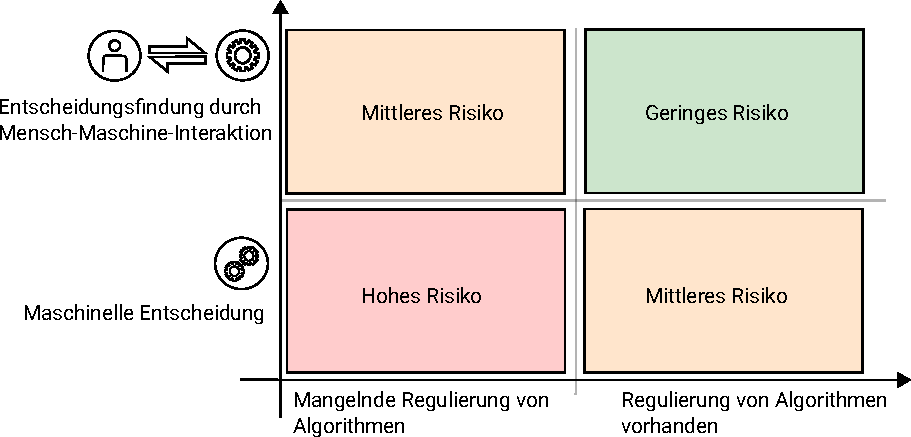
\includegraphics[scale=1.0]{Grafiken/Risk_Matrix_Ink.pdf} 
\label{pic:Risiko_Matrix}
\end{figure}

Zudem sollte es keine grundsätzlichen technologischen Probleme bei der Einführung von
Predictive Analytics geben. Grundlegende statistische Methoden sind bereits in
Tabellenkalkulationsprogrammen verfügbar, für erweiterte Anwendungen existieren zahlreiche
Varianten von Programmbibliotheken (siehe Anhang~\xcom) und Data Warehouse Lösungen sind
ebenfalls für den öffentlichen Sektor erhältlich (vgl. \cite{IT_Novum}, S.~11).

%-------------------------------------------------------------------------------

%In diesem Zusammenhang sind auch verschiedene Interpretationen des
%Wahrheitsbegriffs bedeutsam. Eine weit verbreitete Interpretation wird mit
%Hilfe des Pragmatismus von William James definiert (vgl. \cite{Precht}). Demnach werden
%Aussagen von Menschen als Wahrheit akzeptiert, falls die Aussagen ihnen bei der
%Orientierung in der Welt nützlich sind. Dies liefert eine Erklärung dafür, dass
%Menschen dazu tendieren Aussagen zu glauben, die ihre eigene Weltsicht
%bestätigen. Bei einer extremen Ausprägung des pragmatischen Wahrheitsbegriffs
%wird aus der Nützlichkeit einer Aussage ihr Wahrheitsgehalt abgeleitet:
%\glqq{Es ist wahr, weil es nützlich ist}\grqq.

%Diese radikale Wahrheitsinterpretation ist problematisch, wenn die als Wahrheit
%betrachteten Grundsätze der Realität widersprechen. Denn es gibt keine
%Möglichkeit, die Grundsätze mit Hilfe von empirischen oder logischen Beweisen
%zu revidieren und an die Realität anzupassen. Langfristig führen falsche
%Grundsätze somit zu schlechtem Urteilsvermögen, was wiederum zu schlechten
%Entscheidungen führt. Insbesondere sind Datenanalysen in einer solchen Situation
%nicht zweckdienlich, da Ergebnisse selektiv ignoriert oder abgelehnt werden.

%Eine andere Interpretation von Wahrheit legt großen Wert auf die Beweisbarkeit
%von Aussagen. Eine solche Interpretation ist beispielsweise in der Wissenschaft
%verbreitet. Aussagen wird erst dann ein Wahrheitswert zugewiesen, wenn
%unwiderlegbare Beweise für die Gültigkeit der Aussage vorhanden sind. Eine
%solche Interpretation weicht stark vom pragmatischen Standpunkt ab, kann aber
%ebenfalls problematisch werden. Es besteht die Gefahr sich bei der Prüfung von
%Aussagen in Kleinigkeiten zu verlieren, handlungsunfähig zu werden oder
%nützliche Erkenntnisse zu lange anzuzweifeln\footnote{
%Beispiele für Zweifel, die gefährlich werden, weil sie Fortschritt blockieren
%sind auf Seite~\xcom erläutert.
%}.

%Vermutlich ist für ein gutes Urteilsvermögen ein nüchterner Pragmatismus
%notwendig, bei dem vorsichtig zwischen Nutzen und Wahrheit abgewogen wird und
%auch unangenehme Meinungen als Wahrheit akzeptiert werden können.
%Bedauerlicherweise gerät ein solcher Pragmatismus mit jeder, insbesondere
%politischen, Weltanschauung in Konflikt, die selbst nicht in ähnlicher Weise
%pragmatisch ist.

%-------------------------------------------------------------------------------
Der folgende Text bietet eine dialektische Erörterung der Konfliktfelder, die im
Zusammenhang mit der Einführung von Predictive Analytics oder Forecasting entstehen
können.


\subsection{Eine pessimistische Sichtweise}

Die Einführung formaler Methoden zur Entscheidungsunterstützung kann zu unlösbaren Konflikten führen,
da sie drei Verlustängste bei den betroffenen Personen weckt: Verlust von Privilegien,
Verlust der Arbeit und Verlust der kollektiven Einheit. 

\begin{description}
\item[(1) Verlust von Privilegien:] \hfill \\
Die Einführung einer evidenzbasierten Methode entzaubert den Entscheidungsträger\footnote{
Hier wird vereinfacht angenommen, dass eine Person die Urteile fällt und die Entscheidungen
trifft. Die Ausführungen sind aber auch auf Gruppen von Entscheidern (Entscheidungsgremien)
anwendbar.
}, da sie die Schwächen seiner Urteile offenbart. Die typischen Rechtfertigungsmuster
(Belief System Defenses, siehe S.~\xcom)
sind dann nicht mehr anwendbar.

\item[(2) Verlust der Arbeit:] \hfill \\
Der Entscheidungsträger verliert seine Arbeit an jemanden, der besser mit den neuen Methoden
arbeiten kann. Diese Gefahr ist besonders dann groß, wenn in der Organisation eine Arbeitsteilung
zwischen Spezialisten (vgl. \cite{Gluchowski}, S.~107), die Datenanalysen bereitstellen und Informationskonsumenten
(vgl. \cite{Gluchowski}, S.~105-106), die die Informationen für Entscheidungen verwerten, besteht. 
Da die Spezialisten, mit einer mathematiknahen Ausbildung, besser mit den Methoden umgehen können, 
können sie die bisherigen Entscheidungsträger ablösen.

Je mehr das Treffen von Entscheidungen zu den Haupttätigkeiten von Personen
gehört, desto stärker betrachten sie Predictive Analytics als Gefahr für ihren
Arbeitsplatz. Aus diesem Grund ist zu erwarten, dass das Führungspersonal auf der taktischen
und strategischen Ebene solche Reformen am stärksten bekämpfen wird. Weiterhin wird sich Predictive
Analytics am leichtesten auf der operativen Ebene etablieren lassen, da operatives Management meist
auch andere Tätigkeiten wahrnimmt, auf die es sich dann stärker konzentrieren kann. Zudem verfügen
operative Kräfte nicht über so viel Macht wie taktische oder strategische Entscheidungsträger.

\item[(3) Verlust der kollektiven Einheit:] \hfill \\
Der evidenzbasierte Charakter von Forecasting und Predictive Analytics bedroht die Stabilität
von (politischen) Weltanschauungen.
Tetlock kam bei seiner Studie zu dem Urteil, dass die Kernaufgabe politischer Weltanschauungen
nicht die Erstellung möglichst korrekter Prognosen ist, sondern die
Aufrechterhaltung einer bequemen Illusion von Berechenbarkeit
(vgl. \cite{Tetlock}, S.~39). Die Stabilisierung von Glaubenssätzen, die zum
kollektiven Zusammenhalt beitragen, erhält also eine höhere Priorität.
Dabei kann die investigative Art von Datenanalysen Nervosität und Unbehagen auslösen und als
subversiv wahrgenommen werden. Politische Faktoren spielen im öffentlichen Sektor eine größere Rolle als
im privaten Sektor und die Themengebiete sind kontroverser. Aus diesem Grund ist davon auszugehen, dass
evidenzbasierte Methoden im öffentlichen Sektor, zumindest auf taktischer und strategischer Ebene,
ein heikles Thema sind. 

\end{description}

Die Verlustängste überwiegen in diesem Szenario so stark, dass eine Einführung
evidenzbasierter Methoden strikt abgelehnt wird. Die Einführung findet dann
entweder gar nicht statt, oder die Erkenntnisse werden ignoriert.

\subsection{Eine optimistische Sichtweise}

Die zentrale Motivation dafür evidenzbasierte Methoden in einer Organisation
einzuführen, ist die Möglichkeit zu erhalten, bessere Entscheidungen zu treffen.
Dies bringt sowohl Vorteile gegenüber Konkurrenten als auch Vorteile beim
\glqq{Spiel gegen die Natur\grqq{} (siehe S.~\xcom). So sind beispielsweise Staaten Stammkunden
für Prognosen und Urteile von Experten (vgl. \cite{Roetheli}, S.~256) und haben damit ein
starkes Interesse daran, diese zu verbessern. Es gibt auch Impulse, die direkt aus den Nachrichtendiensten
kommen. Schon 1951 hat der CIA-Analyst Sherman Kent\footnote{
Wegen seiner Verdienste auf diesem Gebiet wird Sherman Kent als der Vater der modernen
nachrichtendienstlichen Tätigkeit bezeichnet (\emph{father of the modern intelligence profession},
vgl. \cite{Ford}).
} vorgeschlagen, dass der Grad der Unsicherheit einer Prognose in Zahlen anstatt vager Formulierungen
ausgedrückt werden soll (vgl. \cite{Roche}, S.~144 und insbesondere \cite{Kent}).
Allerdings ist damals niemand auf seinen Vorschlag eingegangen. Auch Nick Hare
arbeitete im Auftrag des britischen Verteidigungsministeriums an der Verbesserung von Analysen und
Prognosen (vgl. \cite{Burton}). Das Problem ist, dass die Berichte der Analysten in erzählendem Stil
geschrieben sind und nicht konkret genug, dass nachträglich entschieden werden könnte, ob deren Prognosen
eingetreten sind oder nicht (vgl. \cite{Burton}). So besteht das traditionelle Vorgehen darin, einer
Person mit Expertise auf dem Gebiet nachrichtendienstliche Berichte zu präsentieren und ihre Einschätzungen
aufschreiben zu lassen. Eine nachträgliche Kontrolle ihrer Genauigkeit findet nicht statt. Diese Probleme
können mit evidenzbasierten Methoden vermieden werden.

Weiterhin kann interner Druck die Ängste negieren.
Das Festhalten an Privilegien auf Kosten der Allgemeinheit ist eine
egoistische Handlung und birgt langfristig viel Konfliktpotential. Personen, die die
Harmonie aufrechterhalten wollen, werden dem Druck nachgeben. 

Nicht alle Gruppen oder Kulturen haben die gleichen Probleme mit kollektiver Identität.
Manche Gruppen können mit evidenzbasierten Methoden besser umgehen als anderere.
Zudem können die Gefahren amgemildert werden, indem loyale und ideologisch motivierte
Personen mit der Durchführung beauftragt werden. Diese sind vertraut mit den
Besonderheiten und Tabus einer Weltanschauung und können diese umgehen.

%-------------------------------------------------------------------------------
%Bessere Prognosen und Urteile führen zu besseren Entscheidungen. Dies bringt
%wiederum sowohl Vorteile gegenüber Konkurrenten als auch Vorteile bei der
%Auseinandersetzung mit der \glqq{Natur}\grqq\footnote{
%Genauer: Bei der Auseinandersetzung mit den Zwängen, die durch die Naturgesetze
%und ökonomische Prinzipien definiert werden. Verzichtet man zum Beispiel auf das 
%Rauchen kann es als eine gute Entscheidung betrachtet werden, da man dadurch
%gesünder lebt. Hierfür muss zunächst erkannt werden, dass Rauchen ungesund ist.
%Klingt heute einfach. Diese Erkenntnis zu erlangen war jedoch mit erheblichem
%Aufwand verbunden, wobei auch wissenschaftliche und statistische Methoden
%eine große Rolle spielten (vgl. zum Beispiel \cite{Proctor}).

%Ein weiteres Beispiel für eine Entscheidung, die nicht in erster Linie Vorteile
%gegenüber Konkurrenten verspricht, ist eine Entscheidung für eine bessere
%Behandlungsmethode in der Medizin. Denn der primäre Zweck davon ist, 
%mehr Menschen eine Heilung zu ermöglichen.
%}
%-------------------------------------------------------------------------------
Der Wille, bessere Entscheidungen zu treffen, überwiegt in diesem Szenario, während
die Ängste abgemildert oder ganz aufgehoben werden.

\section{Spieltheoretische Betrachtung}

% traditionelle vs progressive Spieler

Aufgrund der potentiell konfliktreichen Situation rund um die Einführung von
Forecasting und Predictive Analytics, bietet es sich an, die
\gls{glos:Spieltheorie} anzuwenden. Es werden einfache spieltheoretische Modelle
präsentiert, die die obigen Szenarien verdeutlichen sollen.

\subsection{Einleitung zur Spieltheorie}
% TODO
% name metaphorisch

\subsection{Das pessimistische Szenario}
% deadlock (S. 218(
\begin{figure}%[!hbt]
\centering
\caption{Deadlock Auszahlungsmatrix}
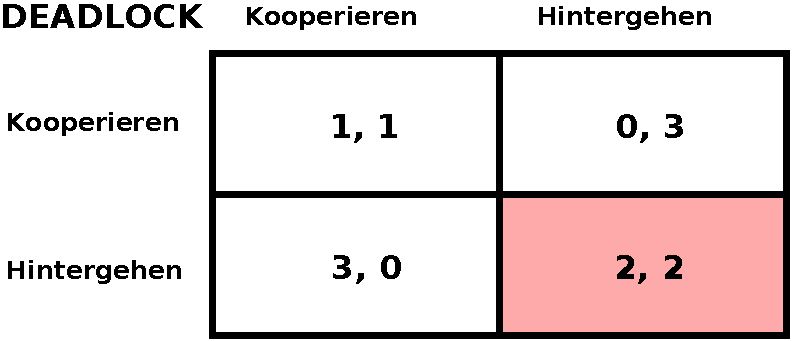
\includegraphics[scale=0.8]{Grafiken/Deadlock_Ink.pdf} 
\label{pic:Deadlock}
\end{figure}


\subsection{Das optimistische Szenario}
% stag hunt (S. 220)
\begin{figure}%[!hbt]
\centering
\caption{Stag Hunt Auszahlungsmatrix}
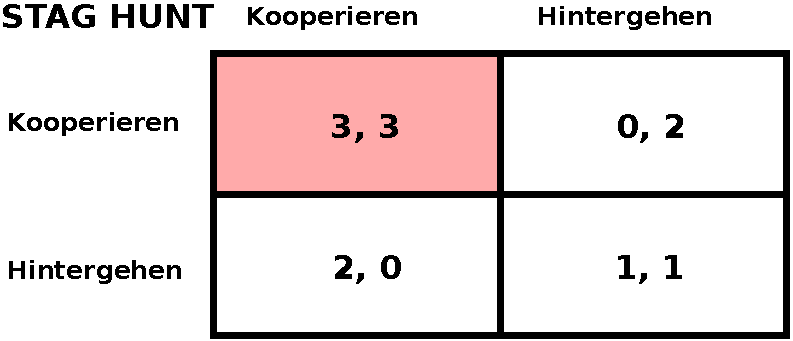
\includegraphics[scale=0.8]{Grafiken/Stag_Hunt_Ink.pdf} 
\label{pic:StagHunt}
\end{figure}

\subsection{Gemischtes Szenario}
% mixed
\begin{figure}%[!hbt]
\centering
\caption{Gemischte 'Stag Hunt - Deadlock' Auszahlungsmatrix}
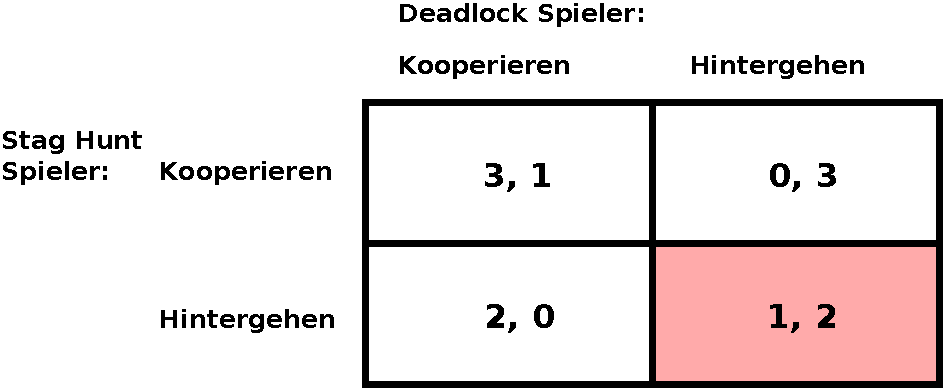
\includegraphics[scale=0.8]{Grafiken/Mixed_Ink.pdf} 
\label{pic:Mixed}
\end{figure}

\subsection{Kritische Würdigung der spieltheoretischen Betrachtung}

\subsubsection{Alternative Spielvarianten}

% TODO spielen implizit spieltheorie (s. Poundstone ?)

% prisoners dilemma (S.237)
% mixed
\begin{figure}%[!hbt]
\centering
\caption{Gefangenendilemma Auszahlungsmatrix}
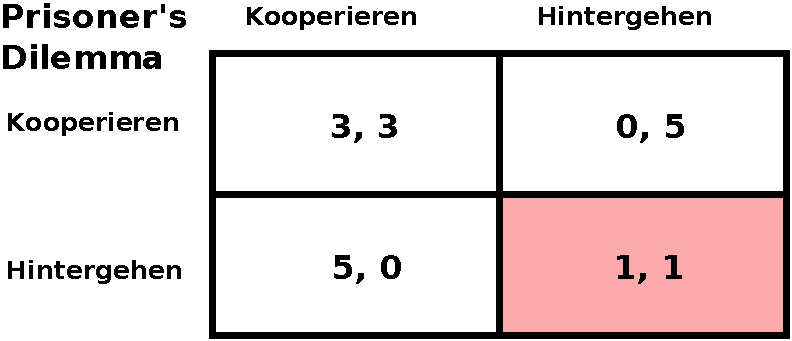
\includegraphics[scale=0.8]{Grafiken/Prisoner_Ink.pdf} 
\label{pic:Prisoner}
\end{figure}